\documentclass[12pt]{article}
\usepackage[a4paper, margin=1in]{geometry}
\usepackage{times}
\usepackage{graphicx}
\usepackage{tikz}
\usetikzlibrary{shapes.geometric, arrows.meta, positioning, calc}
\usepackage{cite}
\usepackage{setspace}
\usepackage{titlesec}
\usepackage{hyperref}

\onehalfspacing

\titleformat{\section}{\large\bfseries\scshape}{\thesection.}{1em}{}
\titleformat{\subsection}{\normalsize\bfseries}{\thesubsection.}{1em}{}

\begin{document}

\begin{center}
    {\LARGE \textbf{DefectLens: Efficient ViT-Based Anomaly Detection with Multi-Criteria Token Fusion (MCTF)} \par}
    \vspace{0.5cm}
    {\large \textbf{Chinmoy Das} \par}
    {\large Roll No: 2023bcs0052 \par}
    {\large Computer Vision Course Project \par}
    {\large Weekly Project Write-Up \par}
    \vspace{0.5cm}
\end{center}

\begin{abstract}
\noindent This write-up delineates the core objectives and underlying architecture of the DefectLens project. It focuses on the computational limitations of applying standard Vision Transformers (ViTs) to high-resolution automated anomaly detection. Furthermore, it details the integration of a Multi-Criteria Token Fusion (MCTF) mechanism designed to facilitate high-speed edge processing, effectively balancing the dual requirements of low-latency inference and high-accuracy defect localization in industrial settings.
\end{abstract}

\vspace{0.5cm}

\section{Problem Statement}
Automated visual inspection is a critical component of modern manufacturing quality control. Traditional supervised machine learning techniques are inherently limited because they require extensive, labeled examples of every potential defect. Because manufacturing anomalies are rare and highly varied, obtaining such data is practically impossible. Consequently, the industry relies on unsupervised anomaly detection, where models are trained exclusively on normal, defect-free data.

Vision Transformers (ViTs) have recently emerged as state-of-the-art architectures for this task, excelling at capturing both global structural context and local patch details. However, a major drawback of ViTs is their immense computational requirement, which scales quadratically with the number of tokens (image patches). In industrial contexts that demand low latency and high-resolution imaging, processing every single token---most of which represent identical background areas---creates a severe processing bottleneck.

The fundamental problem this project addresses is: \textit{How can we significantly reduce the computational overhead of Vision Transformers for anomaly detection without discarding the high-resolution, localized visual features necessary to pinpoint minute defects?}

\section{Motivation and Real-World Application}
The inability to promptly detect microscopic manufacturing flaws can lead to severe product failures, extensive recalls, and significant safety hazards, particularly in high-precision industries such as semiconductor fabrication and aerospace engineering. Conversely, an inspection algorithm that is too computationally heavy will throttle the entire production line. Addressing this latency-accuracy trade-off is essential for the progression of smart manufacturing and Industry 4.0.

Our motivation stems from the rigorous demands of active factory floors, where inspection systems must be simultaneously highly accurate and remarkably fast. While older Convolutional Neural Networks (CNNs) often fail to grasp complex global textures, unmodified ViTs are far too sluggish to run on real-time edge processing units.

\textbf{Intended Application:} The DefectLens system is explicitly designed to be embedded within Automated Optical Inspection (AOI) setups directly on production lines. By utilizing this highly optimized anomaly detection pipeline, manufacturers can automatically identify structural imperfections, surface contaminants, and assembly errors (similar to those present in the MVTec AD dataset) in real-time as products are transported along high-speed conveyors.

\section{Project Objectives}
The primary objective of the DefectLens project is to develop a streamlined, high-throughput industrial anomaly detection framework that leverages the superior feature extraction of Vision Transformers while systematically bypassing their computational slowness. The specific objectives are as follows:

\begin{itemize}
    \item \textbf{Baseline Construction:} Develop a foundational Vision Transformer architecture coupled with a PatchCore-inspired Memory Bank to facilitate robust unsupervised anomaly detection.
    \item \textbf{Token Fusion Implementation:} Incorporate a Multi-Criteria Token Fusion (MCTF) module that actively identifies and amalgamates redundant background tokens across the network layers, utilizing the methodologies described by Lee et al. \cite{lee2023multi}.
    \item \textbf{Feature Protection:} Apply rigorous criteria---including token similarity, one-step-ahead attention, and token size limits---to ensure that the critical visual representations of small defects are not erroneously eliminated during the fusion process.
    \item \textbf{Inference Acceleration:} Dramatically decrease the required Floating Point Operations (FLOPs) and overall processing time by minimizing the active token count, thereby enabling rapid edge inference.
    \item \textbf{System Integration:} Deploy the finalized model within a comprehensive software stack, including a FastAPI backend and a React-based frontend, to simulate an interactive quality control dashboard for factory personnel.
\end{itemize}

\section{System Architecture Diagram}
In order to reduce token count without degrading performance, the MCTF module is integrated between the progressive blocks of the Vision Transformer. Figure \ref{fig:architecture} depicts the comprehensive workflow, starting from high-resolution image input and culminating in an actionable anomaly heatmap.

\begin{figure}[htpb]
    \centering
    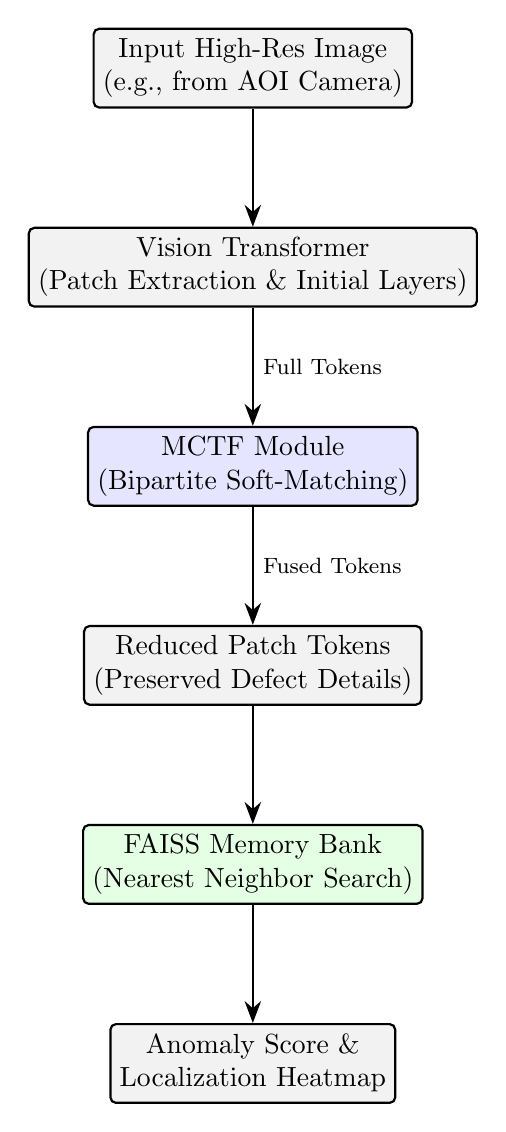
\begin{tikzpicture}[
        node distance=1.5cm and 1cm,
        box/.style={rectangle, draw=black, thick, minimum width=3.5cm, minimum height=1cm, align=center, fill=gray!10, rounded corners=2pt},
        arrow/.style={-{Stealth[scale=1.2]}, thick}
    ]
        % Nodes
        \node[box] (input) {Input High-Res Image \\ (e.g., from AOI Camera)};
        \node[box, below=of input] (vit) {Vision Transformer \\ (Patch Extraction \& Initial Layers)};
        \node[box, below=of vit, fill=blue!10] (mctf) {MCTF Module \\ (Bipartite Soft-Matching)};
        \node[box, below=of mctf] (fused) {Reduced Patch Tokens \\ (Preserved Defect Details)};
        \node[box, below=of fused, fill=green!10] (memory) {FAISS Memory Bank \\ (Nearest Neighbor Search)};
        \node[box, below=of memory] (output) {Anomaly Score \& \\ Localization Heatmap};

        % Arrows
        \draw[arrow] (input) -- (vit);
        \draw[arrow] (vit) -- node[right, font=\footnotesize] {Full Tokens} (mctf);
        \draw[arrow] (mctf) -- node[right, font=\footnotesize] {Fused Tokens} (fused);
        \draw[arrow] (fused) -- (memory);
        \draw[arrow] (memory) -- (output);
    \end{tikzpicture}
    \caption{High-Level Architecture of DefectLens integrating MCTF.}
    \label{fig:architecture}
\end{figure}

\section{Core Ideas and References}
The architectural decisions in this project are heavily inspired by recent breakthroughs in optimizing Vision Transformers. Specifically, the token fusion methodology builds upon the seminal work of Lee et al. \cite{lee2023multi}. Their concept of ``one-step-ahead attention'' serves as a foundational mechanism for determining token informativeness. This allows the network to strategically protect tokens that will be critical in subsequent processing stages, ensuring that the minute details of manufacturing anomalies are preserved throughout the model.

\begin{thebibliography}{9}
\bibitem{lee2023multi}
Sanghyeok Lee, Joonmyung Choi, and Hyunwoo J. Kim,
\textit{``Multi-criteria Token Fusion with One-step-ahead Attention for Efficient Vision Transformers,''}
Department of Computer Science and Engineering, Korea University.
Emails: \{cat0626, pizard, hyunwoojkim\}@korea.ac.kr.
\end{thebibliography}

\end{document}
